\documentclass[main.tex]{subfiles}
\begin{document}

\marginpar{Tuesday\\ 2020-12-15, \\ compiled \\ \today}

We seek an analytic expression for the field lines of the dipolar field: 
%
\begin{align}
\vec{B} _{\text{dip}} = \frac{B_p}{2} \qty( \frac{R}{r})^3 \qty(2 \cos \theta \hat{e}_r + \sin \theta \hat{e}_\theta )
\,.
\end{align}

The field lines are defined by the differential equation 
%
\begin{align}
\frac{ \dd{r}}{ r \dd{\theta }} = \frac{B_r}{B_\theta } &= \frac{ 2\cos \theta ( R / r )^3}{\sin \theta  (R / r)^3} = \frac{2}{\tan \theta }  \\
\frac{\dd{r}}{r} &= \frac{2 \cos \theta \dd{\theta }}{\sin \theta }  \\
\dd{\log r} &= 2 \dd{\log \abs{\sin \theta }}  \\
\log r &= \log \abs{\sin \theta }^2 + C  \\
r &= C \sin^2 \theta
\,.
\end{align}

\begin{figure}[]
\centering
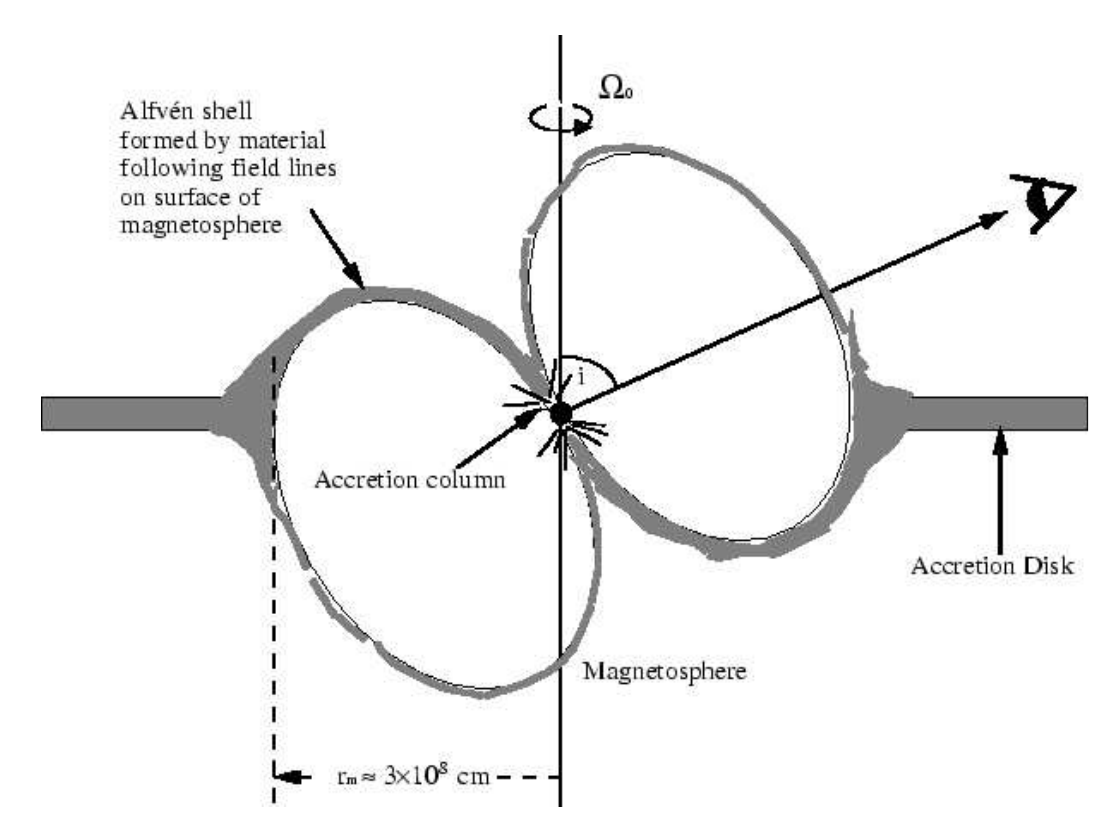
\includegraphics[width=\textwidth]{figures/alfven-accretion}
\caption{A rough sketch of the geometry of accretion onto a NS.}
\label{fig:alfven-accretion}
\end{figure}

We can draw these lines up to the Alfvén radius: the lines reaching that far will reach some point close to the magnetic pole. 
Matter outside this extremal line will be forced to move along field lines.
This means that a lot of the matter will be funneled into a small area near the magnetic poles, as shown in figure \ref{fig:alfven-accretion}. We can compute the size of this area by 
%
\begin{align}
\frac{\sin^2  (\pi / 2)}{r_A} &= \frac{\sin^2\theta_C}{R}  \\
\sin^2 \theta _C & = \frac{R}{r_A} \sim \frac{\SI{10}{km}}{\SI{3000}{km}} \approx \num{3e-3}
\,.
\end{align}

Then, we can compute the critical area \(A_C\): approximating it as a plane disk, we get \(A_C = \pi R^2 \sin^2 \theta _C\), while the total area of the NS is \(A = 4 \pi R^2\): the ratio is then 
%
\begin{align}
\frac{A_C}{A} = \frac{\sin^2 \theta _C}{4} \sim \num{e-3}
\,.
\end{align}

The accretion disk will not be truncated at the surface of the NS, but instead at the Alfvén radius: the matter will be in its thin disk and then be diverted to the poles. 
These regions will reach very high temperatures, and they will source \(X\)-ray emission.

We expect there to be \textbf{accretion columns}: we can write the continuity equation as 
%
\begin{align}
4 \pi R^2 f v \rho = \dot{M}
\,,
\end{align}
%
where \(f\) is a parameter denoting the fraction of area encompassed by the columns (if we evaluate it at the surface of the star it will be the value \(A_C / A \approx \num{e-3}\) we mentioned earlier); the velocity is approximately \(v \sim v _{\text{ff}} = \sqrt{GM/R} = \sqrt{R_S / 2R} \sim c/2\). 
Then, using \(\rho \approx m_p n\), we can express 
%
\begin{align}
n \sim \SI{e16}{cm^{-3}} \dot{M}_{16} f^{-1}
\,.
\end{align}

The mean free path is \(\lambda _D \sim 1/n\) is then on the order of \(\lambda _D \sim \SI{5e11}{cm} \dot{M}_{16}^{-1} f\), much greater than the radius of the NS. 

Therefore, it is \textbf{very difficult for a standing shock to form}, since the particles will not collide for a long distance. 
We compare to the NS radius since we expect the shocks to form near the NS. 

A collisionless shock, on the other hand, can form with \(\lambda _{\text{shock}} \ll \lambda _D\). 
So, only this kind of shock can form. 

The accretion luminosity is 
%
\begin{align}
L _{\text{acc}} &= \eta \dot{M} c^2 = \frac{2GM}{2 R _{\text{NS}}c^2} \dot{M} c^2  \\
&= \frac{R_S}{R _{\text{NS}}} \frac{\dot{M}c^2}{2} \approx \SI{e37}{erg/s}
\,.
\end{align}

This is much smaller than the Eddington limit: one thing we do not need to worry about is the prevalence of radiation pressure. 

There is a redistribution of matter from the poles to the equator, since because of the strong gravity it is very hard to make the NS into a significantly deformed ellipsoid.

\end{document}
